\documentclass[11pt, notitlepage]{report}

\usepackage[tmargin=2cm, lmargin=2cm, rmargin=2cm, bmargin=3cm]{geometry}
\usepackage{parskip}
\usepackage[latin1]{inputenc}
\usepackage{graphicx}
\usepackage{wrapfig}

\begin{document}


\title{MAlice Report}
\author{Owen Davies, Daniel Hertz, Charlie Hothersall-Thomas}
\date{\today}

\maketitle

\section*{The Product}
Our compiler is largely successful and generally meets the criteria set out in the specification for the project. In particular, the syntactic and semantic analysis components of the compiler are extremely sound. There are some small bugs in the code generation portion of the compiler, which we would have liked to fix if we had had more time to spend on the project.

We think that it would be fairly easy to further develop our compiler. Using a class-based system for our AST (with a seperate class for each node) means that it is very easy to add new language features - one can simply add new nodes that extend the \texttt{ASTNode} class, and add methods in the \texttt{TreeWalker} class to create the new node objects. Similarly, in the code generation stage, one can just add new methods to the \texttt{ASTVisitor} class to process the new AST node types. This is one of the benefits of using the visitor pattern to generate code from an AST.

We chose to write our compiler in C++. We made this decision because we wanted to create an object-based solution (to take advantage of design patterns like the visitor pattern), and we also wanted to use this project as an opportunity to further develop our skills in the language - something we feel we have definitely achieved. C++ also has notable performance advantages over other object-oriented languages such as Java. For similar reasons, we chose to compile down to ARM Assembly - ARM is an architecture in which we are all interested (and also one that is growing in popularity very quickly), but not one that we knew much about. We therefore saw this as a good opportunity to learn more about it. We also wanted to take advantage of the Raspberry Pi we had available to use in the project, so compiling down to ARM was the clear option.

Throughout the project we used the \texttt{boost} C++ libraries; in particular \texttt{boost::shared\_ptr} to make memory management simpler (we were initially using raw pointers, but managing these in the semantic analysis stage became very complex). Whilst using \texttt{shared\_ptr}s definitely made the code simpler, they are significantly slower than raw pointers (due to the built-in reference counting). In this case, we decided to sacrifice performance for simplicity.

\section*{Design Choices}
For the lexical and syntactic analysis aspects of the compiler, we decided to use the lexer and parser generator tool \emph{ANTLRv3}. Our success with this tool was mixed due to its steep learning curve, which meant that initial project progress was very slow. \emph{ANTLR} was originally written with Java as a language target. We wanted to use C++, and it soon became apparent that the documentation was distinctly lacking for the C++ target. In fact, the \emph{ANTLR} C++ target was so limited that we decided to use the C target instead, which had more features and fair bit more documentation. We could then write C++ code on top of the generated C code.

This approach proved far more successful, and we were soon making rapid progress through the lexing and parsing of the MAlice language. Once one gets to grips with \emph{ANTLR}, it proves to be an incredibly powerful tool. In particular, two features were found to be very useful:
\begin{itemize}
\item \textbf{Syntactic Predicates} - This feature allows you to tell \emph{ANLTR} to look ahead at the next \emph{n} tokens and check to see if the input conforms to this subrule. If it doesn't, \emph{ANTLR} moves to the next rule. This is written as such:
\begin{center}
	\texttt{rule: (A B C) => x | y}
\end{center}
The above rule says ``If \texttt{(A B C)} holds for the current token stream then do \texttt{x}, otherwise do \texttt{y}''. This feature allowed us to get around any ambiguity in the MAlice language very easily.

\item \textbf{Rewrite Rules} - This allows the user to map an input stream to an output tree. This comes in very handy when creating a parse tree, as you can create imaginary nodes for your parse tree that come in very useful when walking the tree later on:
\begin{center}
	\texttt{rule: a b `.' -> \textasciicircum(TOK a b)}
\end{center}
This creates a new sub-tree in the parse tree with \texttt{TOK} as the root node. This rewrite system is also very useful for defining operator precedence, since you can make the binary operator the root node of its own subtree, and the expression automatically has the correct precedence.
\end{itemize}
If we had to go back and redo the project, we would have looked at more options for lexer and parser generation in C++, to avoid the inital few days of wrestling with \emph{ANTLR}, trying to get it to behave as we wished. However, it is an excellent tool once you start to understand it properly.

We decided to manually write the semantic analysis component of our compiler. We could have perhaps used \emph{ANTLR} for this section as well, but we decided that we didn't have enough time to learn the necessary complex aspects of the tool well enough to create a good solution with them. Additionally, the lectures we had been given on semantic analysis were comprehensive enough so that we felt equipped to hand craft this aspect of the compiler.

As mentioned in the introduction, code generation was implemented using the visitor pattern on our AST nodes. Each \texttt{ASTNode} class has an \texttt{accept} method, which tells its visitor everything it knows about itself after semantic analysis (e.g.\ name, type, enclosing symbol table). The visitor, \texttt{ASTVisitor}, then has a method for each class that extends \texttt{ASTNode}, which calls the relevant accept methods and generates any assembly code required for the program.

\section*{Beyond the Specification}
\subsection*{Optimisations}
We have made a number of optimisations in our compiler:
\begin{itemize}
\item \textbf{Removing unecessary \texttt{mov} instructions and sequences} - any instructions of the form \texttt{mov ri ri} and instruction sequences of the form \texttt{mov ri rx ... mov ry ri} are removed.
\item \textbf{Removing uncalled functions} - any functions with are not called in the program (and hence are dead code) are removed from the program code.
\item \textbf{Removing empty statement blocks} - any \texttt{perhaps}, \texttt{either}, or \texttt{eventually} code blocks without a body are removed. This removal is done before code generation to avoid generating code which will later be removed.
\item \textbf{Register allocation} - Before the instructions for an expression are generated, we apply a weighting algorithm to the expression tree which attempts to work out the ``cost'' of each sub expression, and therefore the most sensible order to allocate registers for the expression (we want to generate code for the ``cheapest'' expression first). Expressions like \texttt{(2 * x + y) + x} would normally get evaluated left to right, but it's more efficient to generate code for the right hand side first in this case. We also make sure that two registers never hold the same expression, to try and prevent the program from running out of registers for as long as possible.
\end{itemize}

\subsection*{Extension - Hardware IO in MAlice}
Since we had already decided to compile down to ARM assembly, and had a Raspberry Pi to hand, we thought that it would be fun to extend MAlice to have commands for hardware IO. This was possible due to the GPIO (general-purpose IO) registers present in an ARM microcontroller such as the Pi. We therefore wrote new MAlice commands to control the GPIO pins on the Raspberry Pi. The following MAlice code shows the new commands included in our extended version of MAlice:

\begin{verbatim}
###include io
The looking-glass hatta()
opened
    x was a number.

    The Caterpillar blew out 4 smoke rings. ### make IO4 an output pin
    The Caterpillar inhaled 17 times.       ### make IO17 an input pin

    Alice discovered x through door 17.     ### x = 0 or 1, depending on IO17's value

    17 said Tweedledee.                     ### set pin IO17 high
    Alice slept for 100 milliseconds.       ### sleep for 100ms
    17 said Tweedledum.                     ### set pin IO17 low
closed
\end{verbatim}

The implementation of these features required changes to almost every element in the project, and this is where our design came into play, as it took minimal effort to add commands to the language and get some output. This meant we could spend the majority of the time getting to grips with the Raspberry Pi's (somewhat undocumented) GPIO controller. We implemented setting up the virtual memory to the controllers registers in C, and linked the generated assembly with this library at compile time. This is why \texttt{\#\#\#include io} is needed as the first line of the file, to tell the preprocessor to change the assemble command.

\begin{wrapfigure}{r}{0.35\textwidth}
  \vspace{-20pt}
  \begin{center}
    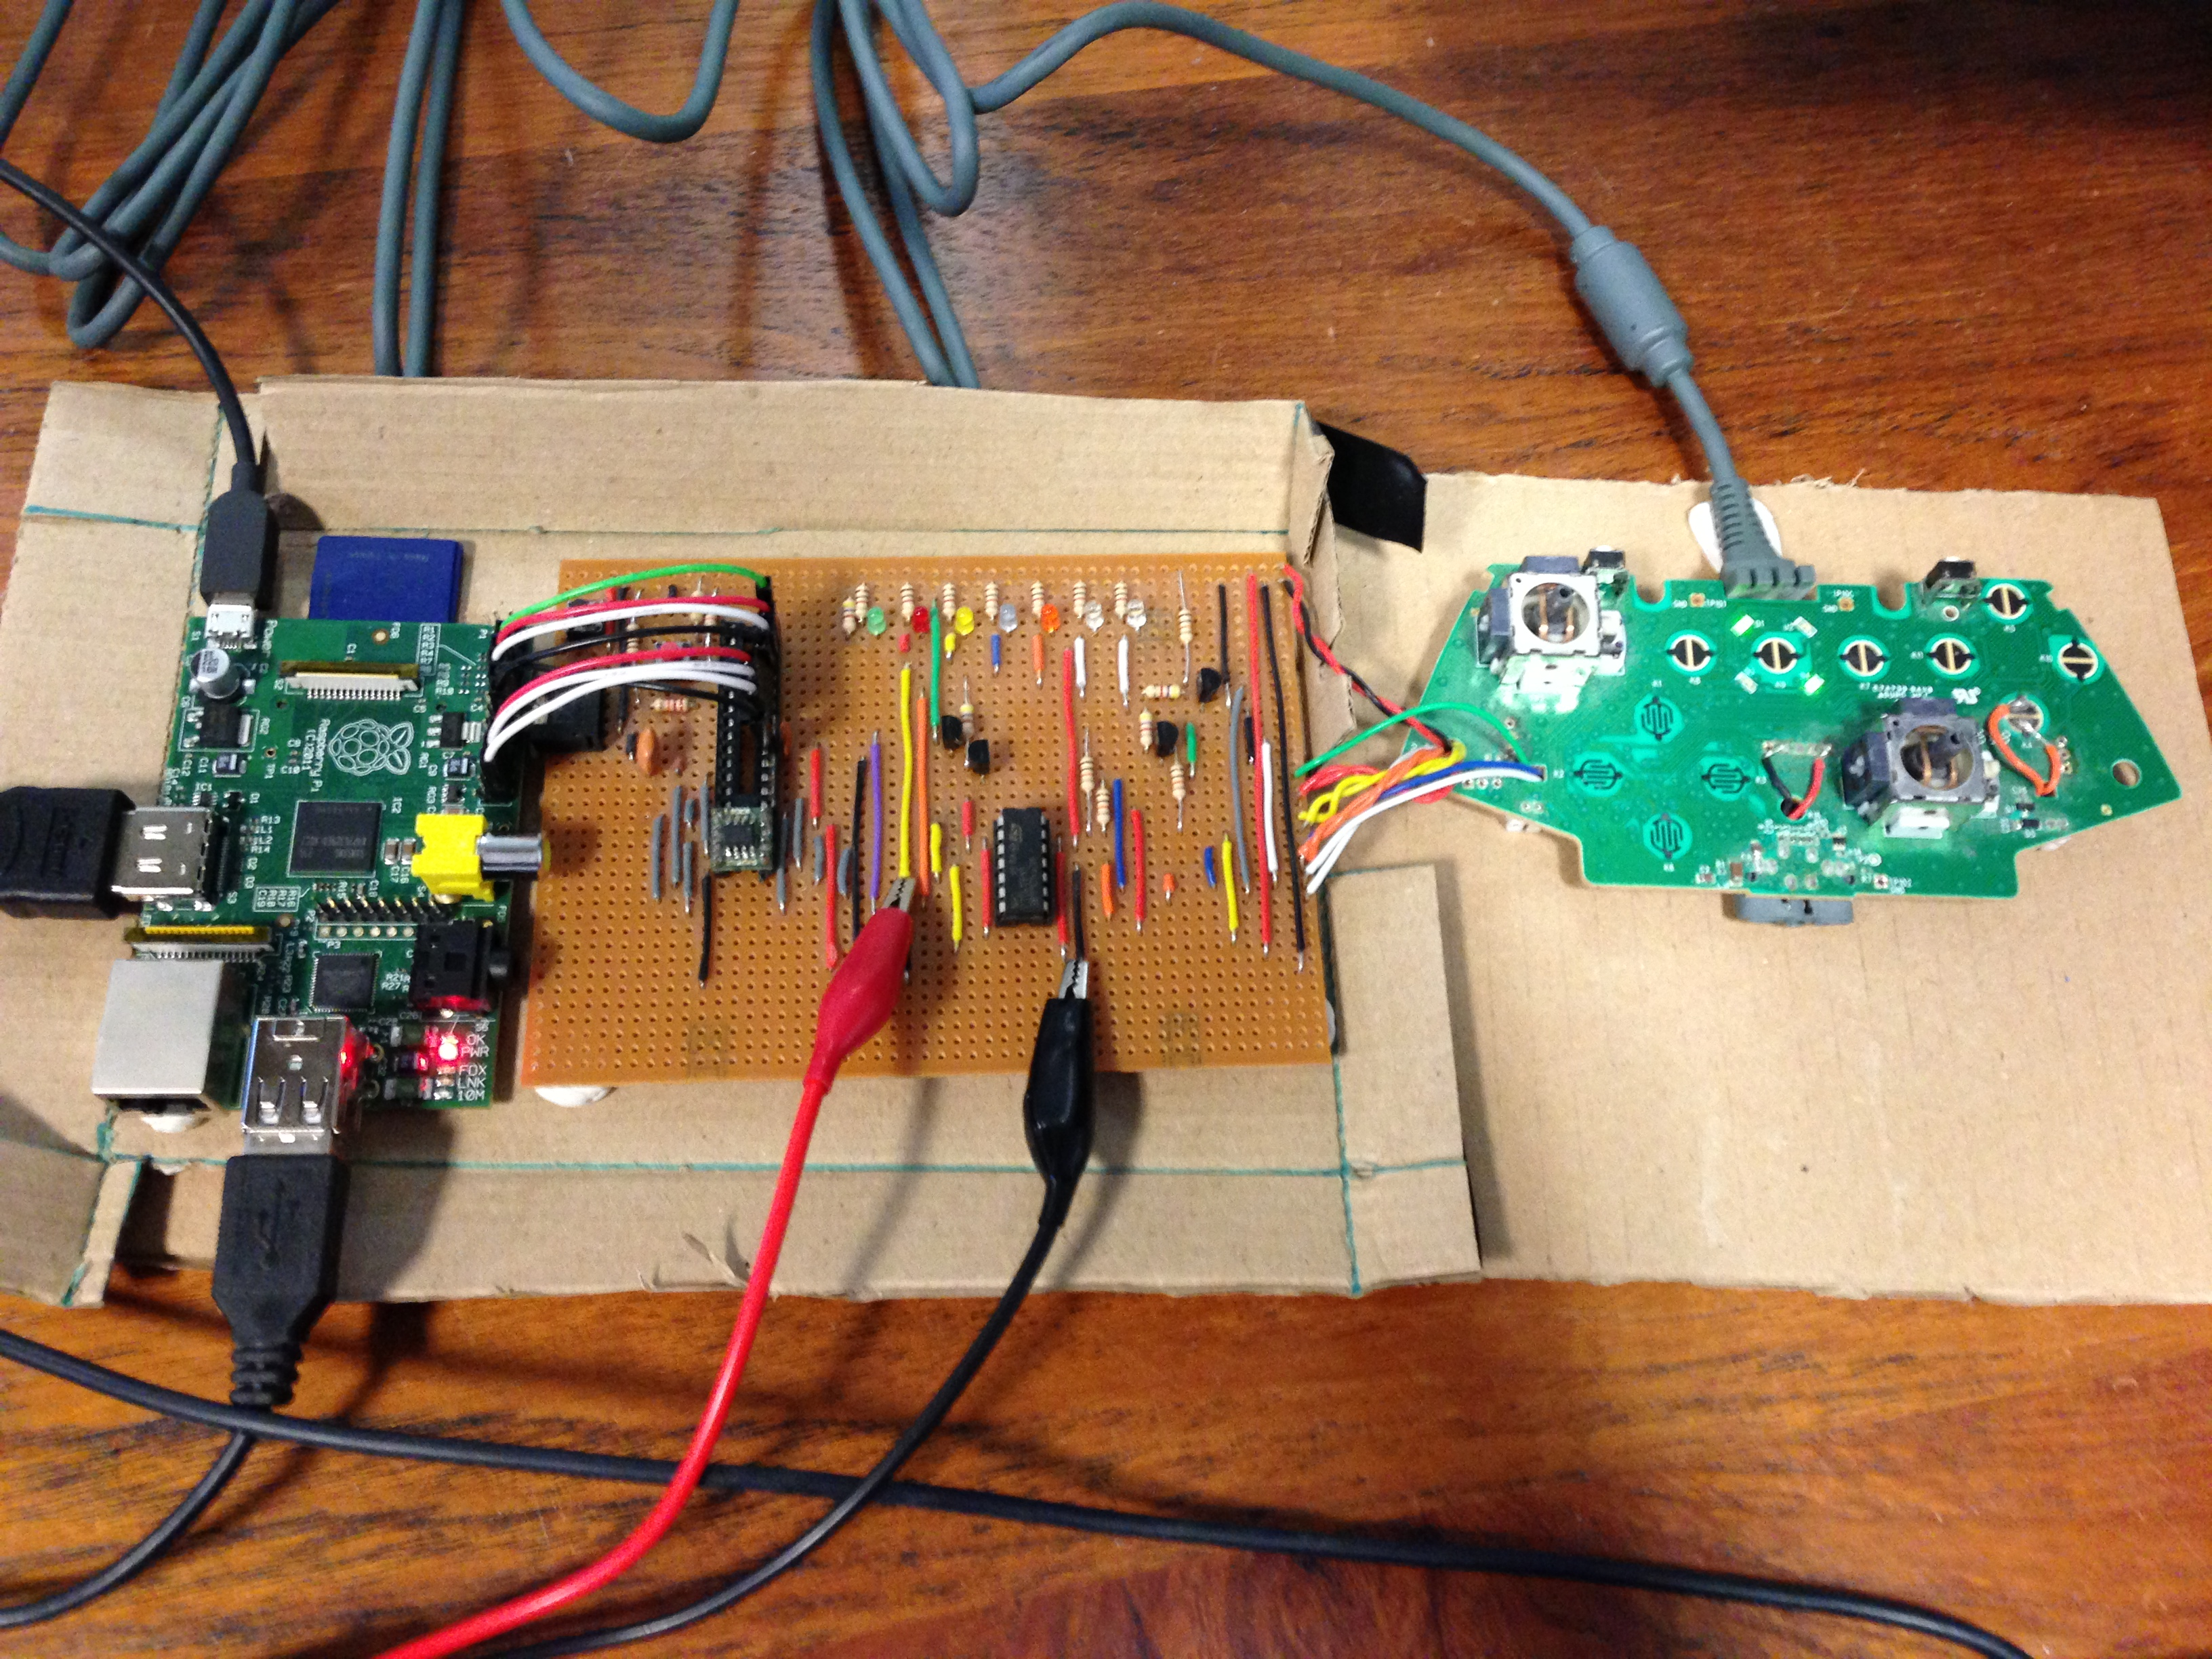
\includegraphics[width=0.35\textwidth]{IMG_9457.JPG}
    \caption{Charlie's awesome circuit}
  \end{center}
  \vspace{-10pt}
\end{wrapfigure}
After the basics had been implemented, we then had lots of fun trying to communicate with the GPIO controller on the lowest level. Our first proof of concept was done in python, with just a LED flashing:

We then wrote out C library to include methods to set pins as input and output, as well as set them high and low. As well as that, we implemented an assembly method to pause the program, so we could then blink an LED.

\begin{wrapfigure}{r}{0.35\textwidth}
  \vspace{-20pt}
  \begin{center}
    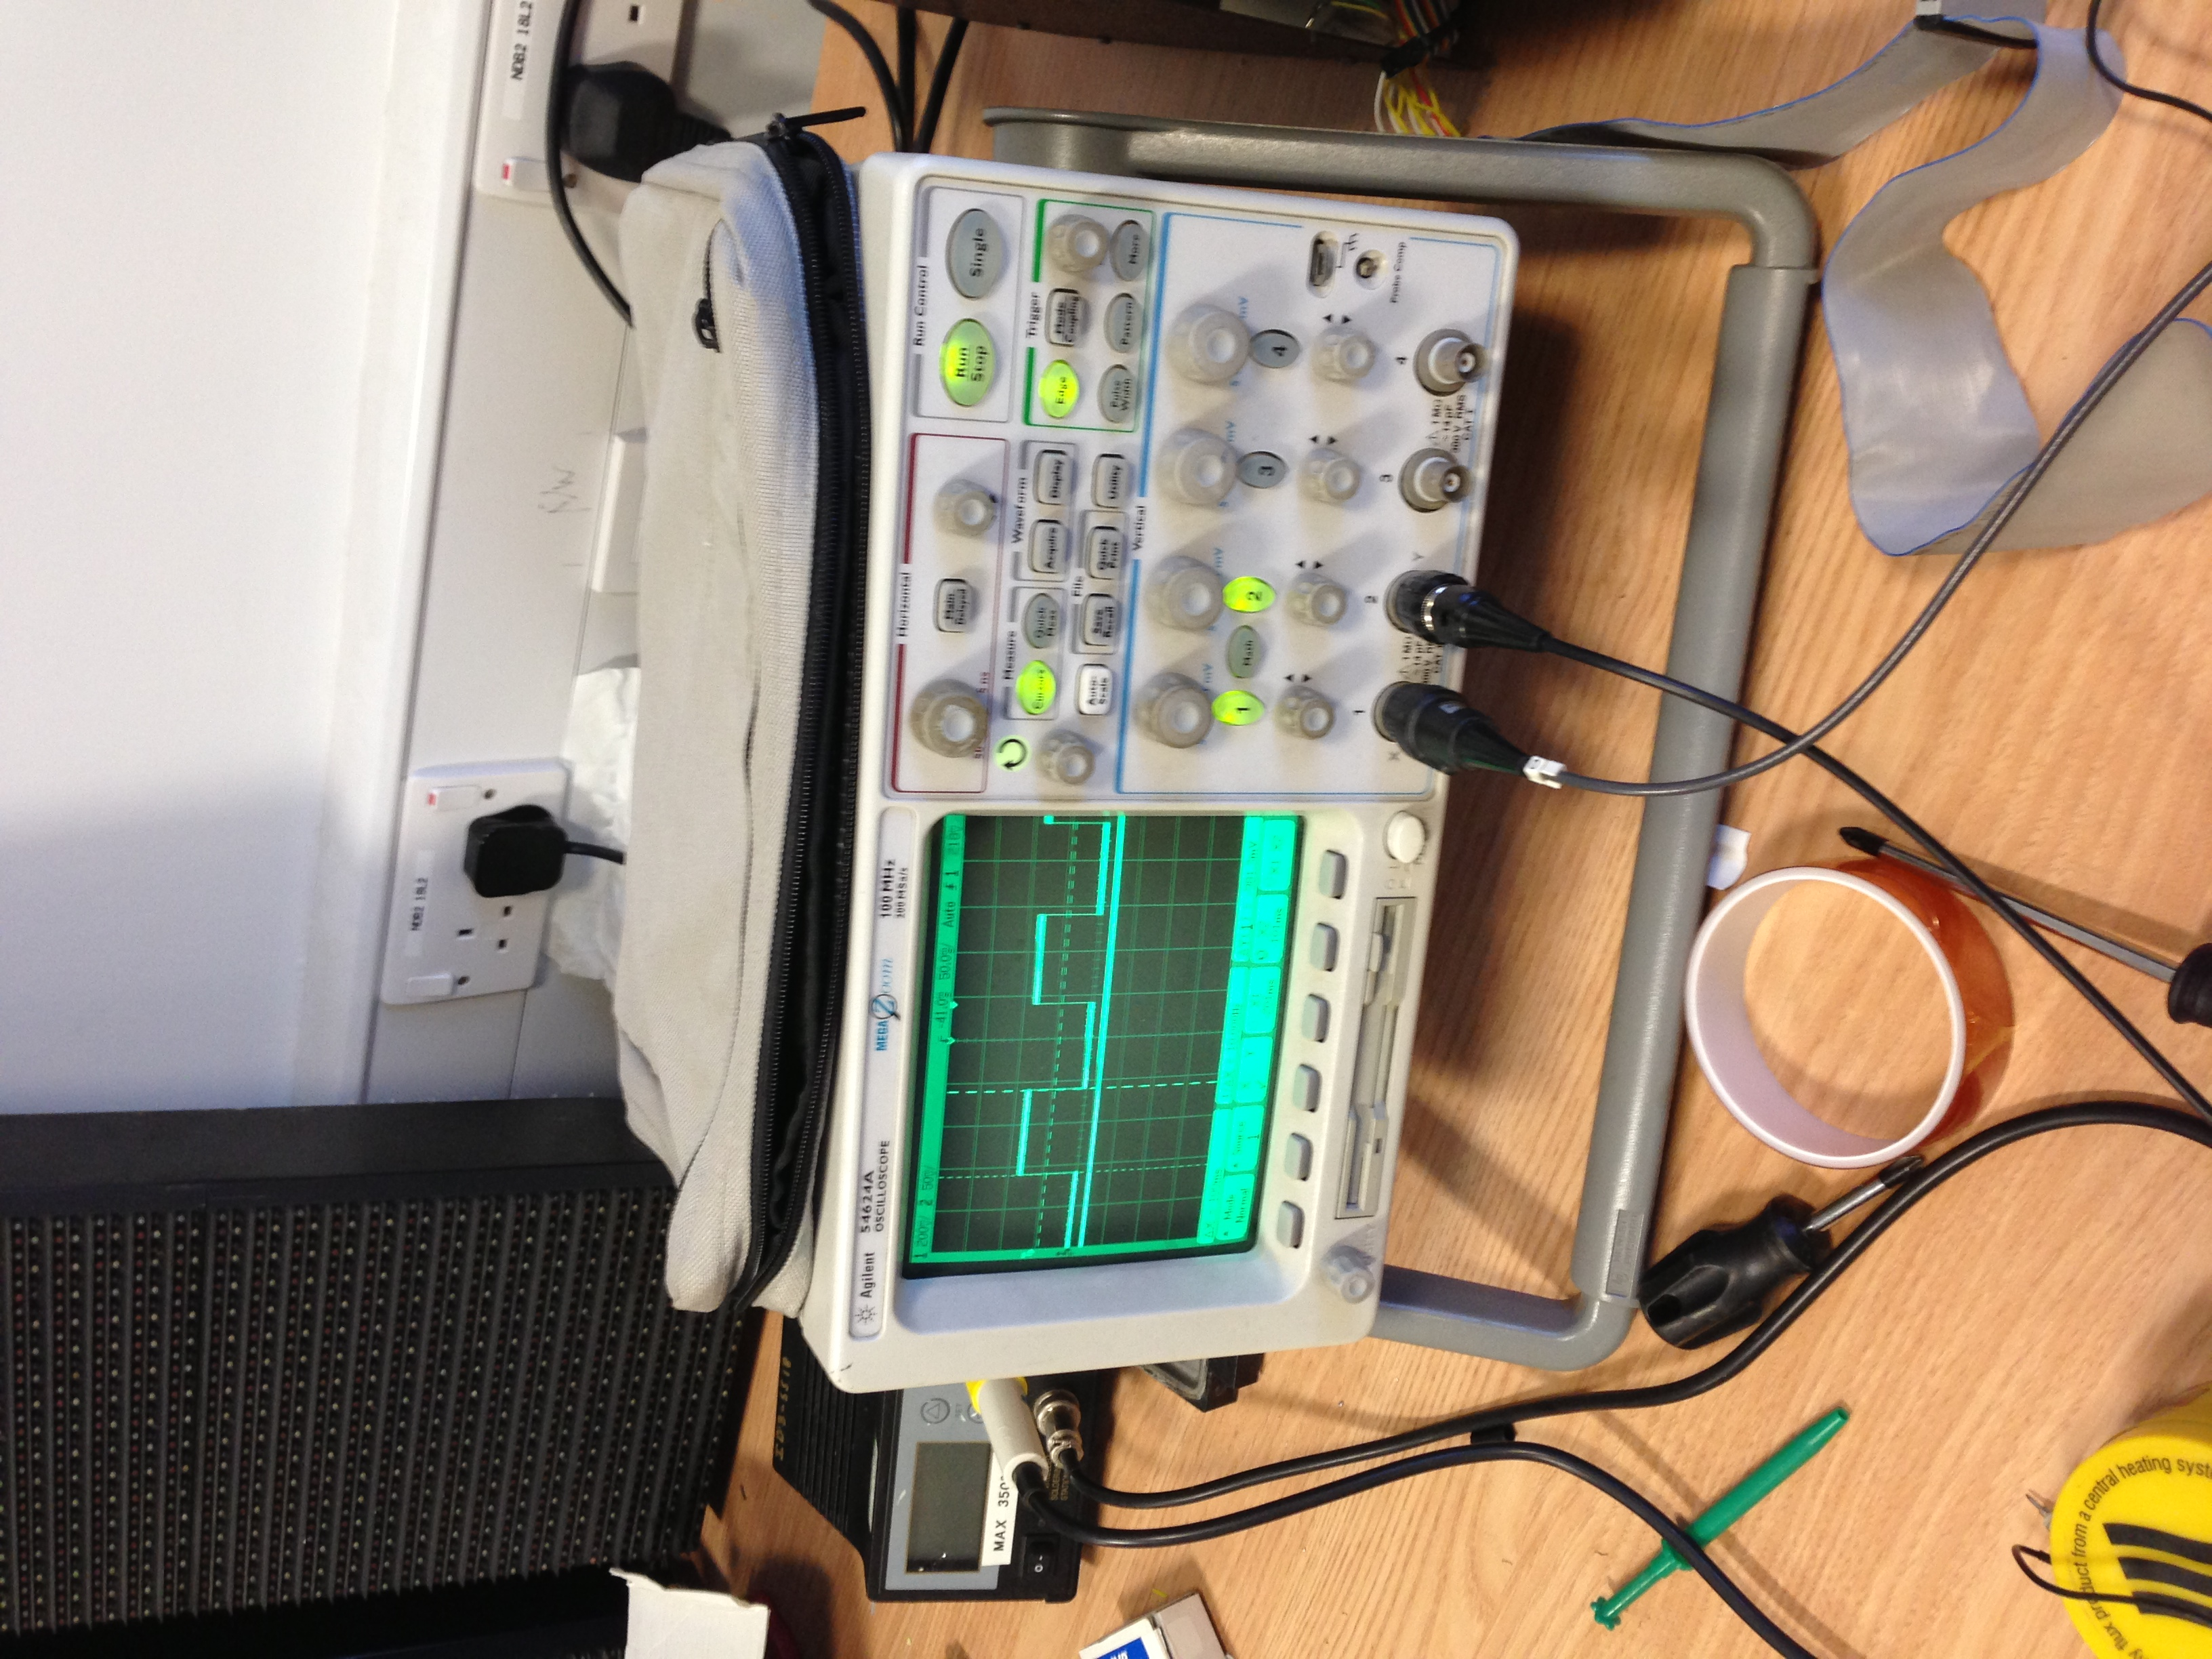
\includegraphics[width=0.35\textwidth, angle=270]{IMG_9458.JPG}
    \caption{}
  \end{center}
  \vspace{-10pt}
\end{wrapfigure}
We then put all these elements together, and to test the new commands, we built some electronics to interface with an Xbox 360, and wrote some malice files to play songs from 'Guitar Hero 3'. During our first effort, the timing of the notes was slightly off, so we asked to use Robotics Society's digital oscilloscope to test our timing code. We then proved that it was millisecond perfect:

This lead to us changing the malice files by eye to account for the mysterious delays in the code, and we had Alice up and rocking.

\end{document}
